\chapter{Resultados Experimentais}
\label{cap:resultados}

Usando o ambiente computacional descrito no capítulo~\ref{cap:implementacao}, foram realizados testes para validar a viabilidade da implementação realizada. Através da criação de dois tipos distintos de aplicações, foi feita uma comparação entre o protótipo na versão sem integração com o PBS (AppMan-RR) com o protótipo integrado ao PBS (AppMan-PBS). 

\section{Aplicações}

Para a realização dos testes e coleta dos resultados foram usados duas aplicações: o algoritmo para \textbf{Cálculo do Fatorial} (Apêndice~\ref{anexo:fatorial}) e o \textbf{Crivo de Eratóstenes} (Apêndice~\ref{anexo:crivo}).

A escolha do algoritmo fatorial se deve ao fato dessa aplicação já constar como exemplo de aplicações usadas no AppMan. Já o crivo é devido a uma necessidade de maior processamento em relação ao fatorial. Além disso o Crivo é um exemplo de aplicação de fato, enquanto que o fatorial é apenas uma forma de forçar o uso de CPU sendo que não serve para resolver nenhum problema em particular.

O Crivo de Eratóstenes é um método para encontrar os números primos de um determinado intervalo informado. Ele retira os números múltiplos dos primos menores que a raiz quadrada (arredondada para baixo) do valor máximo no intervalo informado. O exemplo abaixo demonstra a forma de funcionamento do algoritmo:

Suponha que desejamos a lista dos primos entre 1 e 20. Logo $\sqrt{20} \approx 4,47$, então usa-se 4. 

A lista dos números inteiros até o limite: 2, 3, 4, 5, 6, 7, 8, 9, 10, 11, 12, 13, 14, 15, 16, 17, 18, 19, 20. 

O primeiro primo da lista é o número 2. 

Remove-se todos os múltiplos de 2. Ficando como resultado na lista: 2, 3, 5, 7, 9, 11, 13, 15, 17, 19.

O procedimento é repetido para cada primo encontrado na sequência da lista enquando o valor não exceder a 4 que é o limite estipulado na raíz quadrada. Os valores que restarem na lista são os primos para o intervalo estipulado \cite{Ewerton2008}.

Nos testes realizados no AppMan o intervalo estipulado para cálculo foi de 1 até 10000.

O Fatorial mais divulgado, é o produto de todos os inteiros positivos menores ou iguais a um determinado número (n). Na forma matemática descreve-se como \textbf{n!}. O algoritmo utilizado no presente trabalho funciona da seguinte forma:

É definida uma função recursiva que retorna o fatorial do número propriamente dito: {\bf n! = n*(n-1)!}.

No programa principal existe um laço que faz o cálculo do fatorial de 8 repetir 10000 vezes acumulando esse resultado. Esse laço força o uso de cpu de modo a realizar repetidos cálculos um número de vezes controlado. Essa aplicação pode ser considerada como sintética pois emula uma classe de aplicação sem ser de fato uma aplicação real.

Ambos algoritmos foram desenvolvidos na linguagem \textbf{C}.

Como já existia o algoritmo fatorial nos arquivos do repositório do AppMan, a realização dos testes com o fatorial ocorreu sem problemas. Já com a aplicação crivo, que foi implementada junto com este trabalho, após submeter as tarefas para o protótipo, este demostrou grande quantidade de erros que impossibilitou a execução. Após uma comparação com o código fonte da aplicação fatorial, notou-se que o programa do crivo estava sem o \emph{status} de saída padrão (\textbf{exit(0)}). Após adicionar a saída padrão do programa crivo o funcionamento com o AppMan ocorreu de forma normal.

A métrica utilizada nos testes foi a escalabilidade. Tentou-se submeter o maior número possível de tarefas em ambas as versões do protótipo. A Tabela~\ref{tab:num_max_tarefas} apresenta os números atingidos na submissão das tarefas. No AppMan, para a aplicação Fatorial, foi possível submeter um número máximo 300 tarefas enquanto que no Crivo o número de tarefas submetidas chegou a 250. Já para AppMan-PBS com a aplicação Fatorial o número de tarefas ficou em 200 e com Crivo foi possível submeter 500 tarefas.

\begin{table}[hbtp]
\begin{center}
\caption{Número Máximo de Tarefas Submetidas}
\label{tab:num_max_tarefas}
\begin{tabular}{c|c|c}
	\hline
		& {\bf AppMan-RR} & {\bf AppMan-PBS}\\
	\hline
	{\bf Crivo} & 250 & 500\\ \hline
	\textbf{Fatorial} & 300 & 200\\ \hline
\end{tabular}
\end{center}
\begin{center}
Fonte: Autoria Própria
\end{center}
\end{table}

Como dito anteriormente (capitulo~\ref{cap:implementacao}), o AppMan ainda é um protótipo e seu funcionamento nem sempre é o esperado. Foram necessárias algumas tentativas para chegar ao número máximo de tarefas para cada tipo de aplicação. Erros inesperados ocorreram com certa frequência tornando necessário o reinício de toda a submissão. 

Foi possível atingir números além dos transcridos na tabela~\ref{tab:num_max_tarefas}, porém ao analisar os arquivos de saída notou-se que alguns erros, arquivos necessários para análises não foram gerados completamente. Devido a esse fato essas submissões não foram utilizadas para fins de estatísticas.

\section{Análise do Tempo Total de Execução}

O tempo levado para completar o número de tarefas submetidas é contabilizado pelo próprio protótipo, iniciado no momento que a aplicação recebe o arquivo \emph{DAG} até o final da conclusão e recebimento dos resultados de todas as tarefas submetidas. 

Abaixo temos dois gráficos (~\ref{fig:fatorial_total}, ~\ref{fig:crivo_total}) mais detalhados na Tabela~\ref{tab:tempo_total} demonstram a relação do tempo total de execução com o número das tarefas. Podemos notar que a medida que aumenta o número de tarefas, proporcionalmente o tempo de execução também é aumentado. Esse resultado é o esperado, uma vez que, o aumento de tarefas implica no aumento da complexidade total da aplicação e, portanto, a quantidade de ciclos de CPU necessários para executar a aplicação.

\begin{figure}[htb]
\begin{center}
\includegraphics[scale=0.77]{./img/MapaFatorialTempoTotal.ps}
\caption{Tempo Total \textbf{Fatorial}}
\label{fig:fatorial_total}
Fonte: Autoria Própria
\end{center}
\end{figure}

Ao analisarmos os gráficos~\ref{fig:fatorial_total}, ~\ref{fig:crivo_total} e a Tabela~\ref{tab:num_max_tarefas} é possível notar que não foi possível atingir um número igual de tarefas para todas as combinações de execução. Isto se deve por dois motivos:

\begin{itemize}
	\item As duas aplicações submetidas tem grau de complexidade diferentes.
		É possível verificar que o tempo total de execução da aplicação fatorial é maior que o crivo. Analisando os algoritmos (Anexos ~\ref{anexo:crivo}, ~\ref{anexo:fatorial}) logo podemos verificar que o número de iterações no laço para o algoritmo crivo é bem menor que o fatorial.
	\item O procedimento de retorno dos resultados das tarefas submetidas provenientes do PBS é diferente dos resultados do nó que submeteu as tarefas no AppMan. Quando a troca de recebimento de resultado é feita entre dois AppMans, estes se conversam com melhor sincronia controlando o envio do resultado e evitando congestionamento no nó que recebe os resultados. No caso do retorno das tarefas submetidas para o PBS, não há um controle de sincronização entre o AppMan e o PBS. Devido a essa falta de sincronia, inúmeros erros de \emph{socketConnection} foram reportados na saída de execução do protótipo causando alguns travamentos.
\end{itemize}

\begin{figure}[htb]
\begin{center}
\includegraphics[scale=0.7]{./img/MapaCrivoTempoTotal.ps}
\caption{Tempo Total \textbf{Crivo}}
\label{fig:crivo_total}
Fonte: Própria
\end{center}
\end{figure}
	
\begin{table}[hbtp]
\begin{center}
\caption{Tempo de Total de Execução}
\label{tab:tempo_total}
\begin{tabular}{c|r|r|r|r}
	\hline
		{\bf Nro. Tarefas } & {\bf Crivo (PBS)} & {\bf Fatorial (PBS)} & {\bf Crivo} & {\bf Fatorial}\\
	\hline
	{\bf 50} & 94,82 & 160,47 & 41,92 & 81,13\\ \hline
	{\bf 100} & 485,06 & 314,80 & 203,11 & 209,49\\ \hline
	{\bf 150} & 1171,94 & 1174,95 & 670,86 & 678,97\\ \hline
	{\bf 200} & 2252,85 & 2495,61 & 1409,32 & 1562,86\\ \hline
	{\bf 250} & 3395,77 & -- & 2882,32 & 3148,47\\ \hline
	{\bf 300} & 6486,08 & -- & -- & 5142,64\\ \hline
	{\bf 350} & 11080,86 & -- & -- & --\\ \hline
	{\bf 400} & 14989,90 & -- & -- & --\\ \hline
	{\bf 450} & 21950,33 & -- & -- & --\\ \hline
	{\bf 500} & 28239,04 & -- & -- & --\\ \hline
\end{tabular}
\end{center}
\begin{center}
Fonte: Autoria Própria
\end{center}
\end{table}

Nota-se também que os resultados entre os gráficos (~\ref{fig:fatorial_total}, ~\ref{fig:crivo_total}) se invertem, na aplicação Fatorial foi possível submeter mais tarefas com o AppMan-RR enquanto que, na tarefa Crivo, o AppMan-PBS conseguiu muito mais tarefas. O motivo principal dessa inversão é o tamanho do arquivo de retorno (Tabela~\ref{tab:tam_arquivo}), no Crivo o tamanho é consideravelmente maior que no Fatorial. Os resultados da tarefa Crivo demoram mais para serem enviadas, essa demora auxilia na ausência de sincronia entre o protótipo com o PBS, visto que, o nó que está recebendo os resultados tem um tempo maior de intervalo entre o recebimento entre um arquivo e outro. 
Já nos resultados provenientes da tarefa Fatorial, como os arquivos são inferiores, o envio é de forma muito mais rápida causando problemas com o protótipo quando enviado via PBS. Nesse caso a sincronia entre AppMans facilita no processamento das tarefas.

\begin{table}[hbtp]
\begin{center}
\caption{Tamanho do Arquivo de Resultado}
\label{tab:tam_arquivo}
\begin{tabular}{c|c}
	\hline
		{\bf Aplicação } & {\bf Tamanho (Kb) }\\
	\hline
	Fatorial & 2,0\\ \hline
	Crivo & 525,8\\ \hline
\end{tabular}
\end{center}
\begin{center}
Fonte: Autoria Própria
\end{center}
\end{table}

\section{Tempo de Preparo}